\documentclass[10pt,a4paper]{article}

\usepackage[margin=1in]{geometry}
\usepackage{graphicx}
\usepackage{booktabs}
\usepackage{array}
\usepackage{caption}
\usepackage{enumitem}
\usepackage{hyperref}

\setlength{\parskip}{0.4em}
\setlength{\parindent}{0pt}

\title{Programming Assignment 3: ResNet on CIFAR-100}
\author{20230387 Dongseok KIM \\ Introduction to AI Programming, 2026 Spring}
\date{}

\begin{document}
\maketitle

\section{Model Description}

For this assignment I use \textbf{ResNet-18} from \texttt{torchvision.models}, with the final fully-connected layer replaced by a \texttt{nn.Linear(512, 100)} so that the output dimension matches the 100 CIFAR-100 classes. The 18-layer variant was selected because it is the smallest ResNet whose pretrained ImageNet weights are widely available, which allows a fair comparison between training from scratch and fine-tuning from a strong initialization while keeping the per-epoch training cost manageable on a single GPU (about 21 seconds per epoch with batch size 128 in our environment). The same architecture is used for both the scratch and pretrained settings; only the initial weights of the backbone differ. The trainable parameter count is 11{,}227{,}812.

Because the pretrained checkpoint was trained at $224 \times 224$, I resize the $32 \times 32$ CIFAR-100 images up to $224 \times 224$ for both settings. Using the same input resolution for scratch and pretrained guarantees that any accuracy gap can be attributed to the initialization rather than to architectural differences in the input stem.

\section{Preprocessing and Augmentation}

All images are converted to tensors and normalized with the CIFAR-100 channel statistics $\mu = (0.5071, 0.4866, 0.4409)$ and $\sigma = (0.2673, 0.2564, 0.2762)$. For the training set I apply three augmentations on top of \texttt{Resize(224)}:

\begin{itemize}[leftmargin=*,itemsep=0pt]
    \item \texttt{RandomCrop(224, padding=16)} -- adds translation invariance,
    \item \texttt{RandomHorizontalFlip()} -- doubles the effective training set for left-right symmetric classes,
    \item \texttt{RandomErasing(p=0.25)} -- masks out random rectangular regions and forces the model to rely on multiple discriminative regions rather than a single dominant cue.
\end{itemize}

The 50{,}000 official training images are split into a 45{,}000-image training set and a 5{,}000-image validation set using a fixed random permutation with seed 42. The validation and test transforms are restricted to \texttt{Resize(224)} followed by \texttt{ToTensor} and \texttt{Normalize}, so that the validation signal reflects clean inputs and the test set is evaluated only once on the final best checkpoint.

\section{Pretrained vs.\ Scratch Initialization}

Two initializations are compared under otherwise identical pipelines:

\begin{itemize}[leftmargin=*,itemsep=0pt]
    \item \textbf{Pretrained}: the ResNet-18 backbone is initialized with the \texttt{IMAGENET1K\_V1} weights from \texttt{torchvision}, and only the new classification head is randomly initialized.
    \item \textbf{Scratch}: all weights are randomly initialized with the default \texttt{torchvision} scheme.
\end{itemize}

The difference in convergence speed is striking. With SGD at the per-setting learning rates listed in Section~\ref{sec:results}, the pretrained model reaches a validation accuracy of \textbf{71.88\%} after a single epoch and exceeds 80\% by epoch 6, whereas the scratch model only reaches 16.28\% after epoch 1 and needs more than 40 epochs to pass 70\%. With Adam plus cosine annealing the same pattern holds: pretrained starts at 49.34\% after epoch 1 while scratch starts at 15.00\%.

Final test accuracy follows the same ordering. The pretrained-SGD setting reaches 83.60\% top-1 (97.16\% top-5), while the best scratch run reaches 73.84\% top-1 (93.04\% top-5), a gap of roughly 10 percentage points. The trade-off is that pretrained transfer requires a 45 MB ImageNet weight download, and adapting a pretrained model is less informative if the goal is to study what a deep network can learn end-to-end on a small dataset. Scratch is more flexible and self-contained but pays a clear cost in accuracy and training time under a fixed compute budget.

\section{Learning-Rate Scheduler}

Two schedulers are used in the experiment grid:

\begin{itemize}[leftmargin=*,itemsep=0pt]
    \item \texttt{StepLR(step\_size=10, gamma=0.1)} for the SGD runs. The step decay matches the classical ResNet training recipe, and shrinking the learning rate by $10\times$ every 10 epochs lets the optimizer first explore broadly and then refine.
    \item \texttt{CosineAnnealingLR(T\_max=epochs)} for the Adam runs. Cosine annealing decays the learning rate smoothly from the initial value to zero, which tends to improve final accuracy without requiring tuning of decay milestones.
\end{itemize}

A direct consequence of running for 100 epochs is visible in the \texttt{StepLR} configurations: starting from $10^{-1}$ (scratch) or $10^{-2}$ (pretrained) and decaying by $10\times$ every 10 epochs, the effective learning rate falls below $10^{-7}$ by epoch~60 and below $10^{-12}$ in the final epochs. The per-epoch CSV log of the best run confirms this -- after epoch 51 the validation accuracy oscillates within $\pm 0.2$ percentage points and the training loss barely changes, because the optimizer is effectively frozen. \texttt{CosineAnnealingLR}, in contrast, keeps the learning rate meaningfully above zero until very late in training, so the cosine runs continue to improve over a larger fraction of the schedule. In practice this means that \texttt{StepLR}'s \texttt{step\_size} must be tuned to the total number of epochs, while cosine annealing adapts to the total budget automatically through its \texttt{T\_max} parameter.

\section{Experimental Results}
\label{sec:results}

All experiments use ResNet-18 with batch size 128, weight decay $5\times 10^{-4}$, and seed 42 on a single GPU. Validation accuracy is monitored every epoch, and the test set is evaluated only once using the checkpoint with the highest validation accuracy. Table~\ref{tab:results} summarizes the four primary experiments (100 epochs each); the best validation epoch and top-5 test accuracy are also reported.

\begin{table}[h]
\centering
\caption{Main experiment grid. All runs use ResNet-18, batch size 128, weight decay $5\times 10^{-4}$, and 100 epochs.}
\label{tab:results}
\begin{tabular}{llllrrrrr}
\toprule
Init. & Optimizer & Scheduler & LR & Best Ep. & Val Acc. (\%) & Test Acc. (\%) & Top-5 (\%) \\
\midrule
Scratch    & SGD  & StepLR & 0.100 &  89 & 74.56 & 73.70 & 93.48 \\
Pretrained & SGD  & StepLR & 0.010 &  51 & \textbf{83.62} & \textbf{83.60} & \textbf{97.16} \\
Scratch    & Adam & Cosine & 0.001 &  98 & 74.06 & 73.84 & 93.04 \\
Pretrained & Adam & Cosine & 0.001 & 100 & 78.26 & 77.82 & 94.55 \\
\bottomrule
\end{tabular}
\end{table}

The result table satisfies all four experiment-design requirements of the assignment: it contains at least one pretrained run, at least one scratch run, two distinct learning-rate schedulers (\texttt{StepLR} and \texttt{CosineAnnealingLR}), and two distinct optimizers (SGD and Adam). The best configuration is \textbf{pretrained ResNet-18 with SGD + StepLR, LR $= 0.01$}, reaching 83.60\% top-1 and 97.16\% top-5 on the test set.

For the best run, the five easiest and five hardest classes (by per-class top-1 accuracy on the test set) are:

\begin{itemize}[leftmargin=*,itemsep=0pt]
    \item \textbf{Easiest}: class 94 (98\%), class 58 (97\%), class 75 (97\%), class 68 (96\%), class 8 (95\%).
    \item \textbf{Hardest}: class 47 (67\%), class 55 (66\%), class 72 (62\%), class 11 (59\%), class 35 (58\%).
\end{itemize}

The accuracy spread across classes is roughly 40 percentage points, which is consistent with the fact that several CIFAR-100 super-classes contain visually similar fine-grained categories (e.g.\ the various \emph{small mammals} or \emph{trees}).

\section{Learning Curves}

Figure~\ref{fig:curves} shows the training loss, validation loss, and validation accuracy for the best-performing configuration (pretrained ResNet-18, SGD + StepLR, LR $= 0.01$, 100 epochs). The training loss drops sharply during the first 10 epochs while the learning rate is still $10^{-2}$, then plateaus around 0.09 after the first \texttt{StepLR} decay at epoch 10. The validation loss reaches its minimum around epoch 11 (about 0.58) and the validation accuracy peaks at 83.62\% at epoch 51; after the learning rate falls below $10^{-7}$, both curves remain essentially flat, confirming that further training under this schedule does not help.

\begin{figure}[h]
\centering
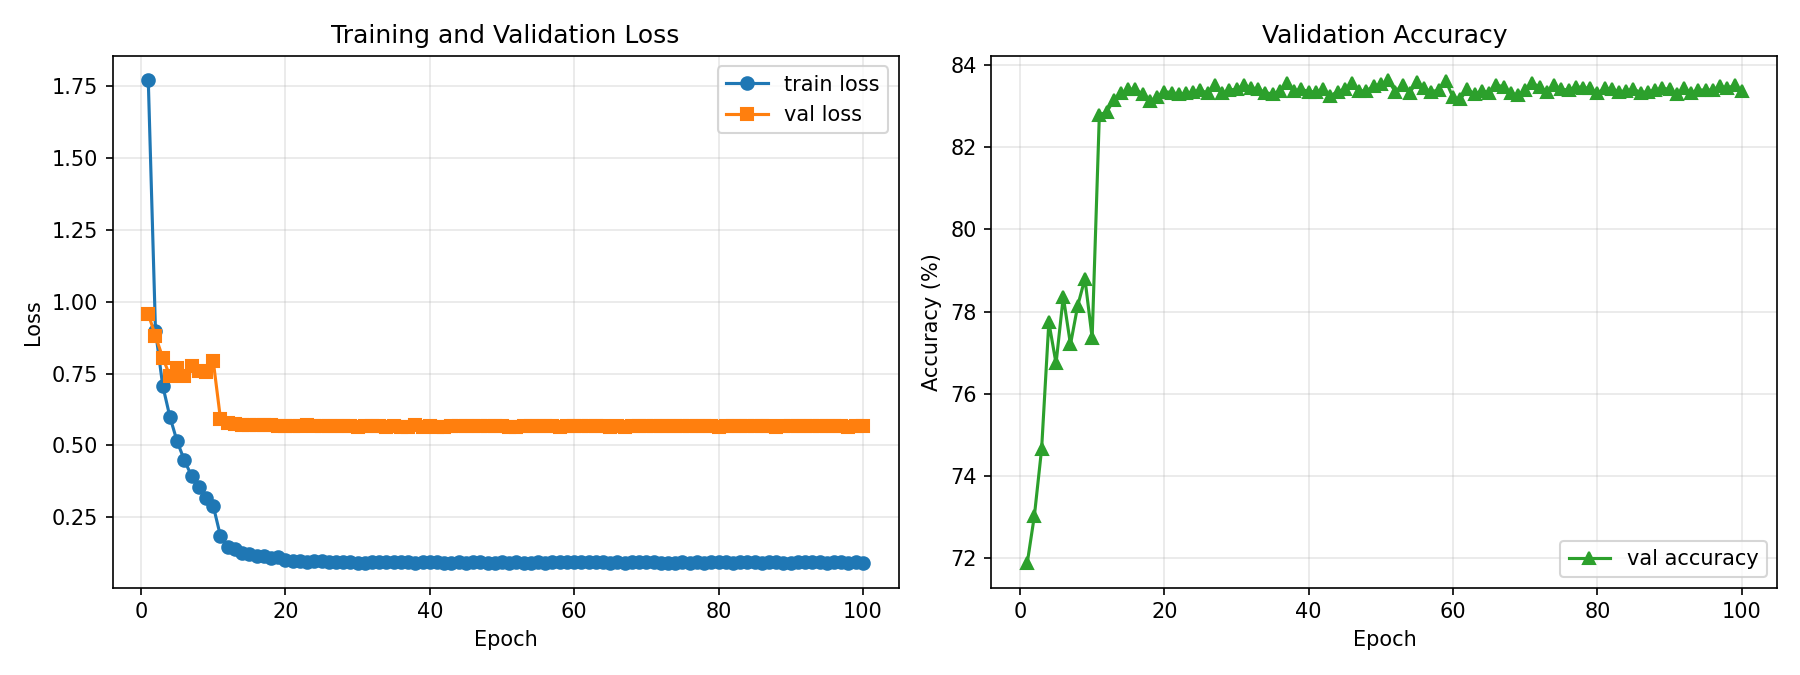
\includegraphics[width=0.95\linewidth]{figures/best_curves.png}
\caption{Learning curves for the best-performing run (pretrained ResNet-18, SGD + StepLR, LR $= 0.01$, 100 epochs). Left: training and validation loss. Right: validation accuracy.}
\label{fig:curves}
\end{figure}

\section{Residual Connection Analysis}

\paragraph{What is a residual connection?}
A residual (or ``skip'') connection adds the input of a block of layers directly to its output: instead of learning a mapping $H(x)$, the block learns a residual $F(x) = H(x) - x$, so that the block computes $y = F(x) + x$. The addition is element-wise and adds no parameters when the input and output dimensions match.

\paragraph{Why are residual connections useful in deep networks?}
They make optimization easier in two ways. First, they create a short, identity gradient path from the loss to every layer, which keeps gradients from vanishing as depth grows. Second, they bias each block toward learning a small correction on top of its input, so adding more layers cannot make the model strictly worse than a shallower one (the optimizer can drive a block's residual function to zero). Together these effects allow networks with dozens or hundreds of layers to be trained without the degradation problem that plagues plain deep networks.

\paragraph{How is ResNet conceptually different from the simple CNN used in Assignment 2?}
The Assignment 2 CNN is a plain stack of convolution, batch normalization, ReLU, and pooling layers, where information flows strictly forward through every layer. ResNet additionally groups layers into residual blocks with skip connections, so each block refines a representation rather than replacing it. This lets ResNet be much deeper (18 layers vs.\ a few) and still trainable, and it changes the role of each block from ``compute the next representation'' to ``compute a small correction to the current one.''

\paragraph{What do the learning curves suggest about optimization difficulty and generalization?}
The smooth, monotonic decrease of the training loss and the rapid drop of the validation loss in the first ten epochs of the pretrained run indicate that optimization is easy: the residual structure plus ImageNet initialization gives the optimizer a well-conditioned starting point. The scratch runs start with a steeper validation loss but still converge, which would be much harder for an equally deep plain CNN. The persistent gap between the final training loss (around 0.09) and the validation loss (around 0.57) on the pretrained run, however, shows that the model has memorized the training set far better than it generalizes, even with weight decay, three augmentation techniques, and a long schedule. This is the residual structure's generalization headroom: the network is easy enough to optimize that it can drive its training loss almost to zero, so further accuracy gains depend on more data or stronger regularization rather than on solving an optimization problem.

\section{Discussion of the Best-Performing Configuration}

The pretrained ResNet-18 with SGD + StepLR (LR $= 0.01$) reaches the highest validation and test accuracy in the grid: 83.62\% validation and 83.60\% test top-1, with 97.16\% top-5. Two factors explain this. First, the ImageNet features are immediately useful for natural images, so the small SGD learning rate of $10^{-2}$ is large enough to adapt the backbone in the first few epochs and small enough not to disturb the pretrained filters. Second, even though \texttt{StepLR} decays aggressively at 100 epochs, this is exactly the regime where pretrained transfer wants a short, sharp adaptation followed by a long, gentle polish -- after epoch 10 the learning rate is already $10^{-3}$ and the model only needs to refine the head.

The scratch runs, by contrast, benefit more from the larger initial SGD learning rate of $0.1$ but cannot fully close the gap in 100 epochs. The scratch + Adam + cosine setting reaches 73.84\% test accuracy, essentially tied with scratch + SGD + StepLR (73.70\%); under the same compute budget the choice of optimizer matters less than the initialization. With a longer schedule, more aggressive augmentation, or a CIFAR-specific stem (smaller first convolution and no initial max-pool), the scratch model could probably reach the high seventies, but it is unlikely to overtake a properly fine-tuned pretrained backbone without substantially more data.

\end{document}
